% \PassOptionsToPackage{quiet}{xeCJK}
\documentclass[fontset=windows, chinese, 10pt]{beamer}

\usepackage{wrapfig}
\usepackage{esint}

% \usepackage{ctex}
\usepackage{xeCJK}
\usepackage{zhnumber}
% \input{../settings/settings_chinese_fonts.tex} % 中文字体设定
\usepackage{tikz}
\usepackage{pgfplots}
% \usepgfplotslibrary{intersections} 

% \uselanguage{chinese}

\usetikzlibrary{quotes,angles}
\usetikzlibrary {arrows.meta}
\usetikzlibrary{decorations.markings}
\pgfplotsset{compat=1.18}

  % \newcommand{\exampletitle}{例题} %

%配合主题，
% \usefonttheme{professionalfonts} 
%和配色包如 
% \usecolortheme{dove}

\usetheme{metropolis}           % Use metropolis theme
% \usetheme{Boadilla}
% \usetheme{Madrid}
% \usetheme{Berkeley}
% \usetheme{Hannover}

% \usepackage{beamerthemeNanjing}
\usepackage{beamercolorthemeHistNanjing}


\newcommand{\red}[1]{\textcolor{red}{#1}}
\newcommand{\blue}[1]{\textcolor{blue}{#1}}
\newcommand{\green}[1]{\textcolor{green}{#1}}
\newcommand{\gray}[1]{\textcolor{gray}{#1}}
\newcommand{\orange}[1]{\textcolor{orange}{#1}}  % orange is supported in xcolor

\include{macro}

\title{复变函数积分}
% \subtitle{A modern beamer theme \textit{摩登主题}}

\date{\zhdigits{2025},\zhganzhinian{2025}年秋}
\author{罗凯}
\institute{南京理工大学物理学院}

% \logo{
  
% 
\includegraphics[height=1cm]{njust-logo.jpeg}

% }

\usebackgroundtemplate{%
\begin{tikzpicture}[remember picture,overlay]
  \node[opacity=0.05, at=(current page.center)] {
    
\includegraphics[width=0.6\paperwidth]{njust-logo.jpeg}
  };
\end{tikzpicture}}

\begin{document}
  % \maketitle

  
  % 好的，我将为你创建一个详细的Beamer幻灯片，专注于第一小节“复数”的内容.每个知识点都会详细展开，包括定义、运算和几何意义.以下是幻灯片的内容：

  % ```latex
  % \documentclass{beamer}
  % \usetheme{Madrid} % 选择一个主题
  % \usepackage{amsmath} % 引入数学公式宏包
  % \usepackage{amsfonts} % 引入数学字体宏包
  % \usepackage{graphicx} % 引入图形宏包
  
  % \title{数学物理方法：复数}
  % \author{罗凯}
  % \date{\today}
  
  % \begin{document}
  
  \begin{frame}
  \titlepage
  \end{frame}
  
  % \begin{frame}{目录}
  % \tableofcontents
  % \end{frame}
  
  \AtBeginSubsection{
    \begin{frame}{目录}
      \tableofcontents[currentsection,currentsubsection]
    \end{frame}
  }

  \section{复变函数积分}
  %%%%%%%%%%%%%%%%%%%%%%%%%%%%%%%%%%%%%%%%%%%%%%%%%%%%%%%%%%%%%%%%
  \subsection{定义和性质}
\label{sec:preknowledge}

\begin{frame}{复变函数的积分}
  \small
有了复变函数微分的基础,我们现在来讨论积分.复变函数的积分的定义可以同实变函数积分的类比得到.
在复平面上取一个路径$\ell$,起终点为$A(z_0),B(z_n)$,沿着该路径定义了一连续函数$f(z)$,用$n-1$个点$z_1, z_2,\cdot, z_{n-1}$将该路径
$\ell$分成$n$个线段(见图\ref{fig:complex_integral}).
函数$f(z)$在线段$z_{k-1}\rightarrow z_{k}$上任意一点$\xi_k$的值乘上线段的长度$\Delta z_k = z_k - z_{k-1}$并求和,即
\begin{equation}
    S_n = \sum_{k=1}^{n} f(\xi_k) (z_{k} - z_{k-1}) .
\end{equation}
\begin{figure}[htbp]
    \centering
    \scalebox{0.6}{
    \input{tikz/integral.tex}
    }
    \caption{复变函数积分示意图.光滑曲线$\ell$上取一系列点$z_k$将其分成$n$小段.}
    \label{fig:complex_integral}
\end{figure}
\end{frame}

\begin{frame}{复变函数的积分}
当$n\to \infty$, 求和则转化为积分.当这个和的极限存在且
与$\xi_k$的选取无关时,这个极限称为
函数$f(z)$沿着路径$\ell$的\textbf{路径积分}(Contour integral), 记作
$\int_{\ell} f(z) dz$,即
\begin{equation}
    \int_{\ell} f(z) dz = \lim_{n\to \infty} \sum_{k=1}^{n} f(\xi_k) (z_{k} - z_{k-1}) . 
\end{equation}
其实,我们还可以将该定义用实虚部的方式表达出来,
\begin{align}
    \int_{\ell} f(z) dz  & = \int_{\ell} \left( u(x,y) + \imath v(x,y) \right) (dx + \imath dy) 
    \\
    & = \int_{\ell} \left( u(x,y) dx  -  v(x,y) dy \right) + \imath \int_{\ell}  \left( v(x,y) dx  + u(x,y)dy \right) 
\end{align}
这样一来,复变函数的路径积分就转化成了两个实变函数的线积分.
因此,很多实函数线积分的性质可以应用在复变函数路径积分上.

\end{frame}

\begin{frame}{积分例子}
\small
\begin{example}
计算积分
\[
\int_{l} z^{2}\,dz
\]
如图所示, 其中终点为 \(A=(2,i)\)，起点为原点 \(O\)。分别沿路径 (1)——从 \(O\) 到 \(A\) 的直线段；
以及路径 (2)——先沿实轴从 \(O\) 到 \(B=(2,0)\)，再从 \(B\) 垂直上升到 \(A\)——计算该积分，并比较结果。

\begin{center}
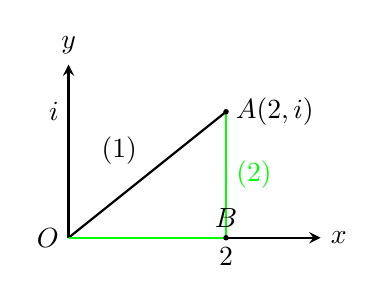
\begin{tikzpicture}[>=stealth,scale=1]
    % 坐标轴
    \draw[->,thick] (0,0) -- (3.2,0) node[right] {$x$};
    \draw[->,thick] (0,0) -- (0,2.2) node[above] {$y$};
    \node[left] at (0,0) {$O$};

    % 点 A 和 B
    \coordinate (A) at (2,1.6);
    \coordinate (B) at (2,0);

    % 路径 (1)
    \draw[thick] (0,0) -- (A) node[midway,above left] {$(1)$};
    
    % 路径 (2)
    \draw[thick,green] (0,0) -- (B) -- (A) node[midway,right] {$(2)$};

    % 标记点
    \fill (A) circle (1pt) node[right] {$A(2,i)$};
    \fill (B) circle (1pt) node[above] {$B$};
    \node[below] at (2,0) {$2$};
    \node[left] at (0,1.6) {$i$};
\end{tikzpicture}
\end{center}


\end{example}




% \onslide<2->{
% \begin{solution}
%   分别沿路径 (1) 和 (2)，如图所示。

% 由复变数定义可得
% \[
% z^2 = x^2 - y^2 + i \, 2xy.
% \]
% \end{solution}
% }

\end{frame}

\begin{frame}{积分例子求解}
\small
\begin{solution}
  \small
先写出复函数的形式
\[
z^2 = x^2 - y^2 + i\,2xy.
\]

\textbf{路径 (1)：} 直线段 \(O\to A\)。

参数化取
\[
z(t)=(2+i)t,\qquad 0\le t\le 1,
\]
因此 \(dz=(2+i)\,dt\) 且
\[
z(t)^2=(2+i)^2 t^2=(3+4i)\,t^2.
\]
于是
\[
\int_{(1)} z^2\,dz
=\int_{0}^{1} (3+4i)t^2\,(2+i)\,dt
=(3+4i)(2+i)\int_{0}^{1} t^2\,dt.
\]
计算常数乘积与定积分：
\[
(3+4i)(2+i)=2+11i,\qquad \int_0^1 t^2\,dt=\frac{1}{3},
\]
因此
\[
\boxed{\;\int_{(1)} z^2\,dz=\frac{2}{3}+\frac{11}{3}i\;.}
\]
\end{solution}
\end{frame}

\begin{frame}
\begin{solution}
  \small

\textbf{路径 (2)：} 分两段，记为 (2a) 和 (2b)。

(2a) 实轴段 \(O\to B\)，参数化 \(z=x\) (\(0\le x\le 2\))，有 \(dz=dx\)，且 \(z^2=x^2\)。于是
\[
\int_{(2a)} z^2\,dz=\int_{0}^{2} x^2\,dx=\left.\frac{x^3}{3}\right|_{0}^{2}=\frac{8}{3}.
\]

(2b) 垂直段 \(B\to A\)，参数化 \(z=2+i y\) (\(0\le y\le 1\))，有 \(dz=i\,dy\)。计算
\[
z^2=(2+i y)^2=4- y^2 + i\,4y.
\]
因此
\[
\int_{(2b)} z^2\,dz
=\int_{0}^{1} (4- y^2 + i\,4y)\,i\,dy
=\int_{0}^{1}\big(4i - i y^2 -4y\big)\,dy.
\]
对每项积分得
\[
\int_0^1 4i\,dy = 4i,\quad
\int_0^1 (-i y^2)\,dy = -\frac{i}{3},\quad
\int_0^1 (-4y)\,dy = -2.
\]
故
\[
\int_{(2b)} z^2\,dz = -2 + \frac{11}{3}i.
\]
\end{solution}
\end{frame}

\begin{frame}
  \small
  \begin{solution}
将两段相加得到路径 (2) 的总积分：
\[
\int_{(2)} z^2\,dz
= \frac{8}{3} + \Big(-2 + \frac{11}{3}i\Big)
= \frac{2}{3} + \frac{11}{3}i.
\]

两条路径的结果一致：
\[
\boxed{\;\int_{(1)} z^2\,dz=\int_{(2)} z^2\,dz=\frac{2}{3}+\frac{11}{3}i\;.}
\]
这符合期望，因为 \(f(z)=z^2\) 在全平面解析，因此对同一端点的曲线积分与路径无关（亦可由柯西定理/原函数原理说明：原函数为 \(F(z)=\tfrac{1}{3}z^3\)）。

\end{solution}
\end{frame}


  %%%%%%%%%%%%%%%%%%%%%%%%%%%%%%%%%%%%%%%%%%%%%%%%%%%%%%%%%%%%%%%%
  \subsection{柯西积分定理}

  \begin{frame}{柯西积分定理}
    柯西积分定理(简称柯西定理)说的是,如果$f(z)$是解析函数,$f'(z)$在闭合路径$C$%构成的单连通
区域内任一点连续,有
\begin{equation}
    \oint_C f(z) dz = 0.
\end{equation}
所有的闭合回路的积分我们用$\oint$来表示.证明会用到格林公式和柯西-黎曼条件,具体参考其他书目,其中
格林公式为
\begin{equation}
    \oint_\ell P dx + Q dy = \iint_S \left( \frac{\partial Q}{\partial x} - \frac{\partial P}{\partial y}  \right) dx dy
\end{equation}

\end{frame}


\begin{frame}{柯西积分定理}
  \small
  对于某些区域有奇点的情况,我们可以取一绕过奇点的闭合路径,如图\ref{fig:complexregion}所示的情况.柯西定理重要的应用在于将沿某一路径积分转化为
另一个或多个路径积分的求和.通常这样来规定正方向,当观察者沿着该方向前进时,区域总是在观察者的左侧.
\begin{figure}
    \centering
    \scalebox{0.6}{
    \input{tikz/complex_region.tex}
    }
    \caption{复杂路径示意图.}
    \label{fig:complexregion}
\end{figure}

  \end{frame}
  

  \begin{frame}{柯西积分定理}
由于$\ell_{in}$和$\ell_{out}$与割线$AB,A'B'$组成了闭合回路,根据柯西定理,我们有
\[
    \left[ \oint _{\ell_{out}} + \int _{\ell_{AB}} + \oint _{\ell_{in}} + \int _{\ell_{B'A'}} \right] f(z) dz = 0 .
\]   
由于割线$AB$与$A'B'$可以无限接近,可以看出二者方向相反,这两项互相抵消.于是我们有
\[
    \left[ \oint _{\ell_{out}} + \oint _{\ell_{in}}  \right] f(z) dz = 0,
\]
即
\[
    \oint_{\ell_{out}} f(z) dz = - \oint _{\ell_{in}}f(z) dz .
\]

\end{frame}

\begin{frame}{复数的极坐标表示}
  若用逆时针方向积分表示,并考虑多个内边界$\ell_{i}$,我们有
\begin{equation}
    \ointctrclockwise_{\ell_{out}} f(z) dz = \sum_{i=1}^{n} \ointctrclockwise_{\ell_{in}} f(z) dz .
    \label{eq:cauchy_integral_summation}
\end{equation}
就是说,外边界逆时针方向积分等于所有内边界逆时针方向积分之和.
只要积分起点和终点固定,当积分路径连续变形时(即不跳过奇点),函数的积分值不变.

下面给出一个重要的例题.
\begin{example}
计算积分\[ I = \oint_\ell (z-\alpha)^n dz, \]其中$n$为整数.
\label{ex:integral}
\end{example}

\end{frame}


\begin{frame}{重要等式}
\small
\begin{solution}
首先,有柯西定理易知,若回路$\ell$不包含$\alpha$,则被积函数在$\ell$所围区域上是解析的,故积分值为零.下面讨论$\ell$包围$\alpha$的情形.
如果$n\geq 0$,被积函数在$\ell$所围区域是解析的,积分为零.若$n<0$,则有一个奇点$\alpha$.取以$\alpha$为圆心半径为$R$的圆周$C$,$R$大小任意.
于是圆周上有$z-\alpha = Re^{\imath \theta}$.
$$
\begin{aligned}
    I &= \oint_\ell (z-\alpha)^n dz\\
     &= \oint_c R^n e^{\imath n \theta} d (\alpha + R e^{\imath \theta})\\
     & =  \imath R^{n+1} \int_0^{2\pi} e^{\imath (n+1)\theta}  d\theta \\
     & = 0 \quad \textrm{if} \quad n\neq -1.
\end{aligned}
$$
\end{solution}
\end{frame}

\begin{frame}{重要等式}
\small
\begin{solution}
当$n = -1$时, $I = 2\pi \imath$.其实,从原函数的角度来看,这个结果很容易理解.当$n\neq -1$,原函数为$(z-\alpha)^{n+1}/(n+1)$, 绕$\alpha$一周
原函数变化量为零.而当$n=-1$时,原函数时$\ln(z-\alpha)$, 绕一周变化量为$2\pi \imath$.因此我们得到了非常重要的表达式
$$
    \begin{aligned}
        & \frac{1}{2 \pi \imath} \oint_l \frac{d z}{z-\alpha}= \begin{cases}0 & (l \text { 不包围 } \alpha), \\
        1 & (l \text { 包围 } \alpha) . \end{cases} \\
        & \frac{1}{2 \pi \imath} \oint_l(z-\alpha)^n d z=0 \quad(n \neq-1) .
        \end{aligned}
$$
\end{solution}
\end{frame}

\subsection{柯西积分公式}

\label{subsec:cauchy_formula}
\begin{frame}{柯西积分公式}

复变函数理论中最重要的一个公式是柯西积分公式.若$f(z)$在一闭合回路围成的区域内解析,$z_0$为区域内一点,
则有
\begin{equation}
    f\left(z_0\right)=\frac{1}{2 \pi i} \oint_C \frac{f(z)}{z-z_0} d z .  
\end{equation}
柯西公式将解析函数在任何一内点 $z_0$ 的值 $f(z_0)$ 用沿边界线 $l$ 的回路积分 表示了出来.
也就是说,一个解析函数在闭合回路$C$内任意点$z_0$的值完全由该路径上的值决定的. 
这看起来不可思议,但又是必然结果.从物理上说, 解析函数紧密联系于平面标量场, 而平面场的边界条件决定着区域内部的场.
我们可以通过前面提到的柯西定理来证明.

我们需要围绕$z_0$选取一个半径为$r$的内圆$\gamma$,由于$f(z)/(z-z_0)$在
内圆与$C$形成的区域解析,故我们有
\[ \frac{1}{2 \pi \imath} \oint_C \frac{f(z)}{z-z_0} d z = \frac{1}{2 \pi \imath} \oint_\gamma \frac{f(z)}{z-z_0} d z
    \]

  \end{frame}

  \begin{frame}{柯西积分公式}
有$z-z_0 = re^{\imath \theta}$,于是
\begin{equation}
    \begin{aligned}
        I &= \oint_\gamma \frac{f(z)}{z-z_0} d z
        \\
        & = \int _0 ^{2\pi} \frac{f(z_0 + re^{\imath \theta})}{re^{\imath \theta}} ire^{\imath \theta} d\theta
        \\
        & = \imath \int _0 ^{2\pi} f(z_0 + re^{\imath \theta}) d\theta
    \end{aligned}
\end{equation}
现令内圆半径$r\to 0$,则有$I\to 2\pi\imath f(z_0)$,得证.
由于$z_0$的任意性,我们可以改写成$z$,而把积分变量改成$\zeta$,则有
      \[
    f(z) = \frac{1}{2\pi \imath} \oint_C \frac{f(\zeta)}{\zeta - z} d \zeta.
\]


  \end{frame}
  
  \begin{frame}{柯西积分公式导数}
    \begin{exampleblock}{柯西积分公式}
        \begin{equation}
            f(z) = \frac{1}{2\pi \imath} \oint_C \frac{f(\zeta)}{\zeta - z} d \zeta.
            \label{eq:cauchy_formula}
        \end{equation}
    \end{exampleblock}


对柯西公式\eqref{eq:cauchy_formula}求导,我们有
\begin{equation}
    f'(z) = \frac{1!}{2\pi \imath} \oint_C \frac{f(\zeta)}{(\zeta - z)^2} d \zeta.
    \label{eq:cauchy_formula_1st_derivative}
\end{equation}
反复求导则有
  
\begin{exampleblock}{柯西积分公式导数}
\begin{equation}
    f^{(n)}(z) = \frac{n!}{2\pi \imath} \oint_C \frac{f(\zeta)}{(\zeta - z)^{n+1}} d \zeta.
    \label{eq:cauchy_formula_nth_derivative}
\end{equation}
    \end{exampleblock}

  \end{frame}
  
\begin{frame}{例题}
 
\begin{example}
  % \small
    计算积分 
    $$ 
    \oint_{\gamma} \frac{1}{z^2 - 1} \, dz  
    $$
    其中 $\gamma$满足$|z| = 2$的闭合路径.
\end{example}
  %   考虑函数 \( f(z) = \frac{1}{z^2 - 1} \)，它在 \( z = 1 \) 和 \( z = -1 \) 处有简单极点.
  %   我们选择半径为 2 的圆 \( \gamma \) 作为积分路径，
  %   如下图所示：
  %   \begin{figure}
  %   \scalebox{0.6}{
  %   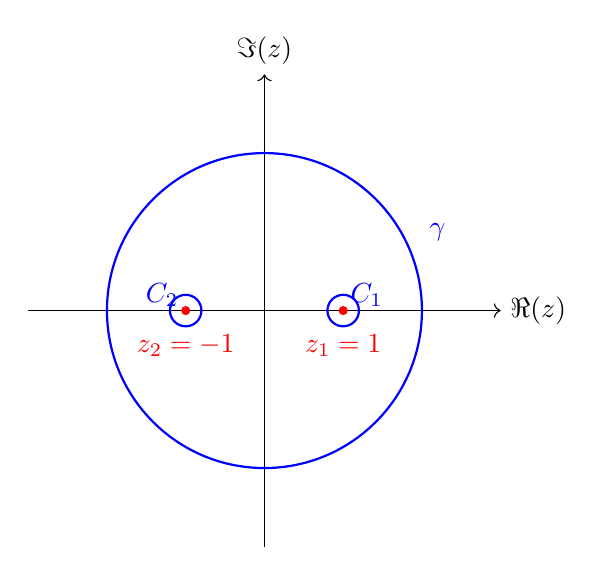
\begin{tikzpicture}[scale=1.0]
        % 画复平面
        \draw[->] (-3,0) -- (3,0) node[right] {$\Re(z)$};
        \draw[->] (0,-3) -- (0,3) node[above] {$\Im(z)$};
        
        % 画半径为2的圆
        \draw[blue, thick] (0,0) circle (2);
        \node[blue] at (2.2, 1) {$\gamma$};
        
        % 标出极点
        \filldraw[red] (1,0) circle (0.05) node[below=5pt] {$z_1=1$};
        \filldraw[red] (-1,0) circle (0.05) node[below=5pt] {$z_2=-1$};
        
        % 绘制绕过 z=1 的小圆弧（顺时针）
        \draw[blue, thick] (1,0) circle (0.2);
        \node[blue] at (1.3,0.2) {$C_1$};

        % 绘制绕过 z=-1 的小圆弧（顺时针）
        \draw[blue, thick] (-1,0) circle (0.2);
        \node[blue] at (-1.3,0.2) {$C_2$};
        
        % 指示方向
        % \draw[->, blue, thick] (1.5,0.5) -- (1.6,0.6);
    \end{tikzpicture}
  %   }
  %   \caption{复平面上闭合路径$\gamma$.}
  %   \end{figure}

\end{frame}


  \begin{frame}{例题}
    \small
    考虑函数 \( f(z) = \frac{1}{z^2 - 1} \)，它在 \( z = 1 \) 和 \( z = -1 \) 处有简单极点.
    我们选择半径为 2 的圆 \( \gamma \) 作为积分路径，
    如下图所示：
    \begin{figure}
    \scalebox{0.7}{
    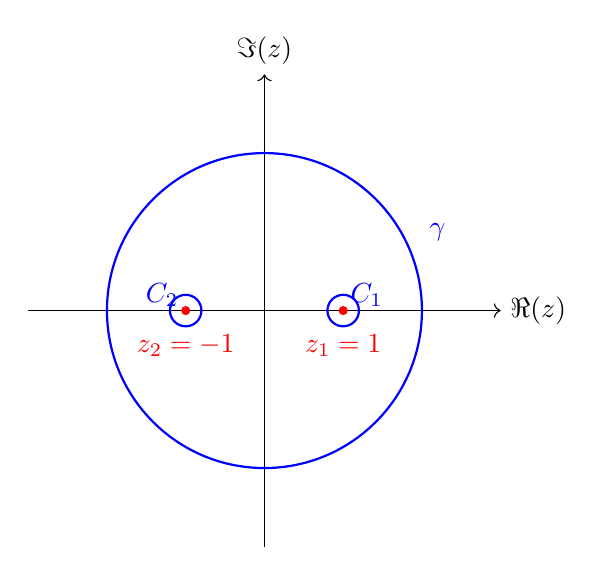
\begin{tikzpicture}[scale=1.0]
        % 画复平面
        \draw[->] (-3,0) -- (3,0) node[right] {$\Re(z)$};
        \draw[->] (0,-3) -- (0,3) node[above] {$\Im(z)$};
        
        % 画半径为2的圆
        \draw[blue, thick] (0,0) circle (2);
        \node[blue] at (2.2, 1) {$\gamma$};
        
        % 标出极点
        \filldraw[red] (1,0) circle (0.05) node[below=5pt] {$z_1=1$};
        \filldraw[red] (-1,0) circle (0.05) node[below=5pt] {$z_2=-1$};
        
        % 绘制绕过 z=1 的小圆弧（顺时针）
        \draw[blue, thick] (1,0) circle (0.2);
        \node[blue] at (1.3,0.2) {$C_1$};

        % 绘制绕过 z=-1 的小圆弧（顺时针）
        \draw[blue, thick] (-1,0) circle (0.2);
        \node[blue] at (-1.3,0.2) {$C_2$};
        
        % 指示方向
        % \draw[->, blue, thick] (1.5,0.5) -- (1.6,0.6);
    \end{tikzpicture}
    }
    \caption{复平面上闭合路径$\gamma$.}
    \end{figure}



  \end{frame}

  \begin{frame}{例题}
    \small
由(\ref{eq:cauchy_integral_summation})可以知道,
    关于路径 \( \gamma \)的积分
    可以转换为由以下两个部分的路径积分
    \begin{itemize}
        \item 绕过 \( z_1 = 1 \) 的小圆弧 \( C_1 \) 半径 \( \epsilon \)，逆时针方向。
        \item 绕过 \( z_2 = -1 \) 的小圆弧 \( C_2 \) 半径 \( \epsilon \)，逆时针方向。
    \end{itemize}

        由前面例题，并利用$\frac{1}{z^2 -1} = \frac{1}{2}\left( \frac{1}{z-1} - \frac{1}{z+1}\right)$
    \[
    \oint_{C_1} f(z) \, dz =\frac{1}{2}\oint_{C_1} \frac{1}{z-1} \, dz =  \frac{1}{2} \cdot 2\pi i  = \pi i
    \]
    类似地，有
    \[
        \oint_{C_2} f(z) \, dz =-\frac{1}{2}\oint_{C_2} \frac{1}{z+1} \, dz =  -\frac{1}{2} \cdot 2\pi i  = -\pi i
    \]
    综合起来:
    \[
        \oint_{\gamma} \frac{1}{z^2 - 1} \, dz = 0.
    \]
    注意,也可以用后面要学到的留数定理来求解.

  \end{frame}
  


  \begin{frame}{例题}
    \small
    \only<1>{
\begin{example}
    计算 
    $$
    I = \oint_\gamma \frac{e^z}{z^n}, 
    $$
    其中, $n\in \mathbb{Z}$, $\gamma$为满足$|z| = 1$的圆.
\end{example}
}
\onslide<2->{
\begin{solution}
    我们需要计算复变函数 \( \frac{e^z}{z^n} \) 在单位圆 \( \gamma \) 上的闭合积分，
    其中 \( n \in \mathbb{Z} \).
函数 \( f(z) = \frac{e^z}{z^n} \) 的奇点位于 \( z = 0 \).
当 \( n \leq 0 \) 时，\( z = 0 \) 是解析点, 根据柯西定理可得积分为零.
当 \( n \geq 1 \) 时，\( z = 0 \) 是奇点, 根据柯西公式(\ref{eq:cauchy_formula_nth_derivative})可计算积分,
$$ I = \frac{2 \pi \imath }{(n-1)!}$$

综上所述，积分的结果为：

\[
I = \oint_\gamma \frac{e^z}{z^n} \, dz =
\begin{cases}
\frac{2\pi i}{(n-1)!}, & \text{如果 } n \geq 1, \\
0, & \text{如果 } n \leq 0.
\end{cases}
\]

\end{solution}
}
\end{frame}


\begin{frame}{例题}
\small
\begin{example}
计算曲线积分
\[
\oint_{l}\frac{e^{z}}{z^{n}}\,dz,\qquad n=0,\pm1,\pm2,\pm3,\dots,
\]
其中 \(l\) 为以原点为圆心、半径 \(1\) 的正向单位圆： \(|z|=1\)。
\end{example}
\onslide<2->
{
\begin{solution}
设 \(m=n\)。若 \(m\ge1\)，则广义柯西公式给出
\[
\oint_{l}\frac{f(z)}{(z-0)^{m}}\,dz=\frac{2\pi i}{(m-1)!}f^{(m-1)}(0).
\]
取 \(f(z)=e^{z}\)，由于 \(f^{(k)}(0)=1\) , $\forall k$,  代入可得。
若 \(m\le0\)，被积函数在圆内解析，积分为零。

综上所述，整合写成分支形式为
\[
\oint_{l}\frac{e^{z}}{z^{n}}\,dz=
\begin{cases}
\dfrac{2\pi i}{(n-1)!}, & n=1,2,3,\dots,\\[6pt]
0, & n=0,-1,-2,\dots .
\end{cases}
\]
\end{solution}

}
\end{frame}


\begin{frame}{模数原理}

下面介绍柯西公式的重要推论.

\textbf{模数原理} $f(z)$在闭区域上解析,$|f(z)|$只能在边界线上取极大值.

由$f(z)^n = \frac{1}{2\pi \imath} \oint_C \frac{f(\zeta)^n}{\zeta - z} d \zeta$,若$|f(\zeta)|$在$C$上极大值为$M$,
$|\zeta - z|$的极小值为$\delta$, $C$的长度为$s$,则
\[
  |f(z)|^n \leq \frac{1}{2\pi} \frac{M^n}{\delta} s  ,
\]
即
\[
    |f(z)| \leq M \left( \frac{s}{2\pi \delta} \right)^{\frac{1}{n}},
\]
令$n\to \infty$,$|f(z)| \leq M$.证毕.

  \end{frame}
  
  \begin{frame}{刘维尔定理}
    \small
   \textbf{刘维尔(Liouville)定理} \quad 如$f(z)$在全平面上解析且有界,则$f(z)$必为常数.

\textbf{证} \quad $f$有界,即$|f(z)| \leq N$, 对$f'(z)$取模,取以$z$为圆心半径为$R$的圆周,可得
\[
  |f'(z)| \leq \frac{1}{2\pi} \frac{N} {R^2} 2\pi R = \frac{N}{R},
\]
由于$R$任意选定,令$R\to \infty$,有$f'(z) \equiv 0$,所以$f(z)$为常数.

刘维尔定理的一个应用是可以证明代数基本定理,即对任意$n$阶多项式(Polynomial)
\begin{equation}
    P(z) = \sum_{k=0}^{n} a_k z^k (n>0, a_n \neq 0)
    \label{eq:poly}
\end{equation}
有$n$个根满足$P(z) = 0$. 它的证明可以通过反证的方法. 假设$P(z)$没有零点,即$P(z)\neq 0$, 则$1/P(z)$是解析
且有界的,根据刘维尔定理可知$1/P(z)$为常数,即$P(z)$为常数,与$a_n\neq 0$矛盾.可以知道,$P(z)$至少有一个根,记为$\lambda_1$,
那么对$P(z)/(z-\lambda_1)$这一$n-1$阶多项式进行上述论证,我们可以降次直至一阶多项式,共计$n$个根,因此$n$阶多项式
有$n$个根.

  \end{frame}
 \begin{frame}{总结}
  \small
柯西积分定理： 解析函数的闭合回路积分为零。

重要结论:
$$
    \begin{aligned}
        & \frac{1}{2 \pi \imath} \oint_l \frac{d z}{z-\alpha}= \begin{cases}0 & (l \text { 不包围 } \alpha), \\
        1 & (l \text { 包围 } \alpha) . \end{cases} \\
        & \frac{1}{2 \pi \imath} \oint_l(z-\alpha)^n d z=0 \quad(n \neq-1) .
        \end{aligned}
  $$



  柯西积分公式及其导数公式
        \begin{equation*}
            f(z) = \frac{1}{2\pi \imath} \oint_C \frac{f(\zeta)}{\zeta - z} d \zeta.
            \label{eq:cauchy_formula}
        \end{equation*}

        \begin{equation*}
    f^{(n)}(z) = \frac{n!}{2\pi \imath} \oint_C \frac{f(\zeta)}{(\zeta - z)^{n+1}} d \zeta.
    \label{eq:cauchy_formula_nth_derivative}
\end{equation*}

 \end{frame}

  
  
\end{document}